% !Mode:: "TeX:UTF-8"

\baselineskip 20pt

\chapter{绪论}
\label{chap:1}

本章首先介绍动态复杂网络社团检测及其演化分析的研究背景以及其在实际应用中的重要意义,然后详细介绍该领域当前国内外研究现状,并基于此提出本文研究内容与创新点,最后总结了本文的章节结构。
 


\section{研究背景与意义}



%背景

自$1998$年小世界网络~\cite{watts1998collective}与无标度网络\cite{albert1999diameter}提出以来,复杂网络及复杂性科学即迎来了长足的发展。复杂网络作为一种数据结构能够更大程度地保留复杂系统各模块间的交互,因此对复杂网络的研究与探索能够帮助人们理解现实世界的运作模式,如人工系统的运作机理如电网\cite{mets2014combining}、水网\cite{bodini2002towards};人类社会的发展模式,如邮件网络传播模式\cite{barnes2024temporal}、科研合作模式\cite{mariani2024collective};自然界的演化规律,如食物链的鲁棒性\cite{dunne2002food}、城市的韧性\cite{zhang2018review}等。针对复杂网络的研究也逐渐发展出多个不同分支,例如链接预测\cite{zhu2016scalable}、异常检测\cite{ahmed2016survey}、社团检测等\cite{kumar2024community}。


%引出静态社团
社团指的是网络中紧密连接的连通子图,是复杂网络分析中的重要统计特征之一。社团检测在现实世界复杂系统的交互模式挖掘中具有重要意义,联通了网络微观节点与宏观网络结构,能够帮助研究者理解网络的结构和功能,在链接预测、网络动力学分析、网络生成、网络控制、网络同步等复杂网络建模的下游任务中均起到了简化网络结构,提升任务效果的作用\cite{kumar2024community,fortunato2016community}。

现实世界的网络往往是动态变化的,因此动态网络社团检测能够更好地帮助理解和挖掘现实世界的演化规律。
动态网络社团检测指的是在动态网络中考虑时序演化信息对每个网络快照进行社团结构识别,根据任务侧重不同可以分为动态社团检测与社团演化分析。动态社团检测侧重于识别动态网络每个快照中节点的社团归属,社团演化分析侧重于社团在时序演化过程中的规律挖掘。社团演化分析往往通过预定义的各种社团事件如社团合并、分裂、扩张、缩小等行为\cite{palla2007quantifying}来对连续快照的社团进行匹配与识别,一定意义上已经脱离了社团检测的范畴而更倾向于数据挖掘,其方法也大多属于启发式地提升社团匹配效果或对社团演化规律的挖掘。动态社团检测则需要建模动态网络的演化模式以更好地识别动态网络每个快照的社团结构,能够支撑如链接预测等下游任务,也能够在动态网络演化模式建模的基础上对社团演化进行分析与挖掘,从而服务于广泛的实际应用\cite{farajtabar2017coevolve,kumar2024community}。例如,基于手机信令数据为城市传染病疫情提供防控措施建议\cite{he2024urban},将手机收发短信及接打电话等行为视为边、将手机视为节点,通过动态网络社团检测来识别城市人群在城市中的移动模式,以此确定对城市中不同人群的防控措施;在学者合作网络中,可以通过将学者视作节点、学者的合作关系视作边,分析学者合作关系的演化挖掘研究者的研究兴趣转移与不同学科的学科交叉情况、预测未来的热门领域等\cite{wu2019large,wang2022weak};另外,利用在线社交媒体数据如X(原Twitter)平台上,将社交媒体账号视作节点、将账号间的交互视作边,也可以通过动态社团检测方法实现对全球事件的实时聚合,在政治、文化等领域均具有重要的作用\cite{ma2024knowledge}。总的来说,针对动态网络的社团检测研究能够建模动态网络的演化模式,社团结构作为动态网络的介观结构,能够帮助学者更好地理解动态网络的演化机理,对人们理解现实世界复杂系统运转模式具有重要意义。

而基于生成模型的社团检测方法能够从网络生成的角度建模从社团到网络微观节点之间的相互作用关系,但现有方法忽略了网络的高阶生成机理,因此难以准确建模动态网络的演化。因此,本课题在随机块模型对动态网络显式建模的框架下,从实证出发建模动态网络演化的高阶模式,提升动态随机块模型的网络演化建模精度与挖掘能力,并从深度生成模型的视角为动态随机块模型的大规模数据应用提供了方法框架。总体上看,本研究关注动态网络社团检测与演化分析问题,扩展了动态随机块模型的动态网络建模精度,提升了动态随机块模型的演化模式挖掘能力,完善了动态随机块模型的大规模数据应用框架,探索了动态网络微观节点、介观社团、宏观网络快照的层次演化机理。





\section{研究现状}

动态网络结构是由连续的网络快照组成,每个快照都可以被视为一个静态网络,因此在动态网络第一个快照的社团检测往往由静态社团检测方法实现,后续网络快照的社团结构根据动态社团检测方法的核心思想而有所区别。因此本节首先简单介绍静态网络社团检测的研究现状,随后介绍动态网络社团检测与动态网络建模的研究现状,并讨论本文研究内容与现有方法的关系与区别。
\subsection{静态网络社团检测研究现状}
社团作为复杂网络的重要结构,在社交网络、合作网络、生物网络等复杂系统所建模的网络中广泛存在且具有重要的现实意义,能够帮助人们深入理解现实世界复杂系统的结构和功能。自$2002$年Gervan和Newman提出社团的概念以来\cite{girvan2002community},一系列的社团检测方法被学者提出,社团作为一种网络的高阶结构(超脱于节点和边的网络中的结构),也被应用于复杂系统功能与结构分析和挖掘任务中。社团指的是网络中紧密连接的连通子图,社团内部的节点间连边稠密,社团间的节点连边稀疏,随着社团检测方法的不断更新与迭代,其方法大致可以分为基于优化的方法、基于动力学的方法、基于生成模型的方法和基于深度学习的方法\cite{fortunato2016community,jin2021survey}。

基于优化的方法的核心思路是通过优化一个度量函数,该度量函数通常是衡量社团结构优劣的指标,以此实现对于复杂网络中社团结构的启发式优化,例如模块度优化、谱优化等。其中收到广泛研究的是模块度优化算法\cite{zhang2009modularity},模块度(modularity)既可以作为衡量社团检测效果的评价指标,也可以作为优化度量函数来进行社团检测。对于度量函数的优化策略则包括全局搜索、模拟退火、梯度优化等\cite{zhang2014scalable,lee2012modularity,JSJA20241121007},不同优化策略的思想也相对统一,即在保证局部最优解的前提下兼顾优化效率。基于动力学的方法的核心思路是在运行复杂网络的动力学过程如扩散过程\cite{jeub2015think}、自旋动力学过程\cite{traag2011narrow}、同步过程\cite{boccaletti2007detecting}等来实现对社团结构的检测,例如基于随机游走的社团检测方法\cite{pons2006computing,JSJA201912008}通过游走过程所经过的节点的集合与社团的基本定义(同一社团内的节点更容易出现在同一组游走序列中),即可以检测出网络中的社团结构;基于生成模型的方法的核心思想是从生成的角度来考虑社团结构在复杂网络的生成过程的角色和地位,将社团结构作为复杂网络中节点和边生成的中间变量来建模复杂网络的生成机制,通过在数据中拟合该生成模型,进而实现社团结构的求解,其代表性方法包括随机块模型\cite{snijders1997estimation}、度修正的随机块模型\cite{karrer2011stochastic}、混合随机块模型\cite{zhang2020struct}等;基于深度学习的方法则属于“两步法”,其核心思想是首先通过基于图神经网络或随机游走的方法获得节点邻域信息的低维表示向量,随后利用k-means等聚类方法获得节点聚类,并将该聚类视为社团,或通过添加正则化项在训练过程中直接获得聚类结果,具有代表性的方法类别包括自编码器\cite{sun2020network}、生成对抗\cite{zhang2020seal}、图卷积神经网络\cite{he2021community}等。上述各方法的优劣对比如表~\ref{chap1:tab:staticmethod}所示。

\begin{table}[htbp]
	\caption{静态复杂网络社团检测方法对比简表}
	\vspace{0.5em}\centering\wuhao
	\label{chap1:tab:staticmethod}
	\resizebox{0.98\textwidth}{!}{
		\begin{tabular}{lp{4cm}p{3cm}p{3cm}cp{2cm}}
			\toprule[1.5pt]
			方法类别 & 核心思想 & 方法优势 & 方法不足 & 代表性工作\\
			\midrule[1.0pt]
			\textbf{基于优化的方法} & 模型通过优化社团结构的度量函数获得网络的社团划分  & 复杂度较低 & 对于噪声更加敏感  & ~\cite{zhang2009modularity,zhang2014scalable,lee2012modularity} \\
			\textbf{基于动力学的方法} & 基于网络动力学过程结合社团的特征实现对社团结构的识别  & 具有更好的通用性 & 结果依赖于初始化,社团结果不稳定 & ~\cite{jeub2015think,traag2011narrow,boccaletti2007detecting} \\
			\textbf{基于生成模型的方法} & 基于统计推断的思想,将社团结构融入网络的生成过程 & 其理论更加完善,且生成模型能够适用于更广泛的下游任务 & 模型复杂度较高  & ~\cite{snijders1997estimation,karrer2011stochastic,zhang2020struct} \\
			\textbf{基于深度学习的方法} & 首先通过表示学习获得节点低维表示,随后利用聚类算法获得社团结构 & 复杂度低、并行化能力强 & “两步法”所获得的聚类结果并不严格符合社团定义 & ~\cite{sun2020network,zhang2020seal,he2021community} \\
			\bottomrule[1.5pt]
		\end{tabular}
	}
\end{table}


而随着社团概念的逐渐发展,重叠社团、层次社团、语义社团的相关概念也被提出,针对现实世界的复杂网络的挖掘与探索也逐渐深入\cite{fortunato2016community,JSJA201912048}。针对复杂网络社团的相关任务也随着应用面的扩大逐渐由社团检测发展,形成了如社团搜索\cite{fang2020survey}、社团匿踪\cite{chen2021community,JSJA20241121007}、社团语义理解\cite{michlmayr2005case}等细分任务。本文主要面向融合时序信息的动态社团检测,相较于静态社团检测更加复杂,维度也从拓扑层面的子图识别进而融合了节点、社团和网络的时序演化维度的建模,因此上述方法由于未考虑时序维度的建模均不能直接应用于动态社团检测与动态网络分析任务。

 


% 传统动态网络社团检测方法可划分为判别式方法与生成式方法,判别式方法专注于对于动态网络社团结构的识别,通过任务导向来设置模型结构,典型方法包括增量聚类、进化聚类等;生成式方法侧重于建模动态网络的生成过程,将社团结构融入网络生成模型中,通过优化模型后验或推断损失函数对模型参数进行求解,典型方法包括随机块模型、动态隐空间模型、非负矩阵分解等。判别式方法效率高,但无法支持网络的生成或演化模式挖掘;生成式方法的参数均具备一定的物理或现实意义,因此能够支持网络的生成或演化模式挖掘,但是需要对模型参数后验进行推断,效率较低。且(挑战1) 

% 随着深度学习的发展与完善,其对大规模数据的处理能力使得针对网络结构的深度学习方法也渐渐成为主流,然而其黑箱特性亦无法支撑。。。挖掘,近年来,深度生成模型。。。。(挑战2) 

\subsection{动态网络社团检测研究现状}

动态网络由连续的网络切片组成,通常被称之为网络快照,每个快照都表示现实世界复杂网络在某个时间段内的网络结构。动态网络的本质是将时间信息融入到网络拓扑中,这对动态网络社团检测提出了更多的挑战,其任务不仅需要识别动态网络每个快照的社团结构,还需要建模动态网络的演化模式。因此动态网络社团检测包含了两个方面的任务,即识别每个快照的社团结构与社团的时序演化分析\cite{rossetti2018community}。大部分现有方法在任务层面往往各有侧重,或直接将二者视为两个独立的问题进行研究。因此动态社团检测的研究内容可以划分成社团检测方法研究(以识别社团结构为主)和社团演化分析(以挖掘社团演化模式为主)\cite{rossetti2018community}。动态网络社团检测相关方法的分类如图~\ref{chap1:fig:dcdclasses}所示,根据思想的不同,动态社团检测方法研究可以划分为即时社团检测、时序权衡社团检测和跨时序社团检测;而社团演化分析则划分为基于结构相似性的方法和基于预定义的方法。
\begin{figure}
    \centering
    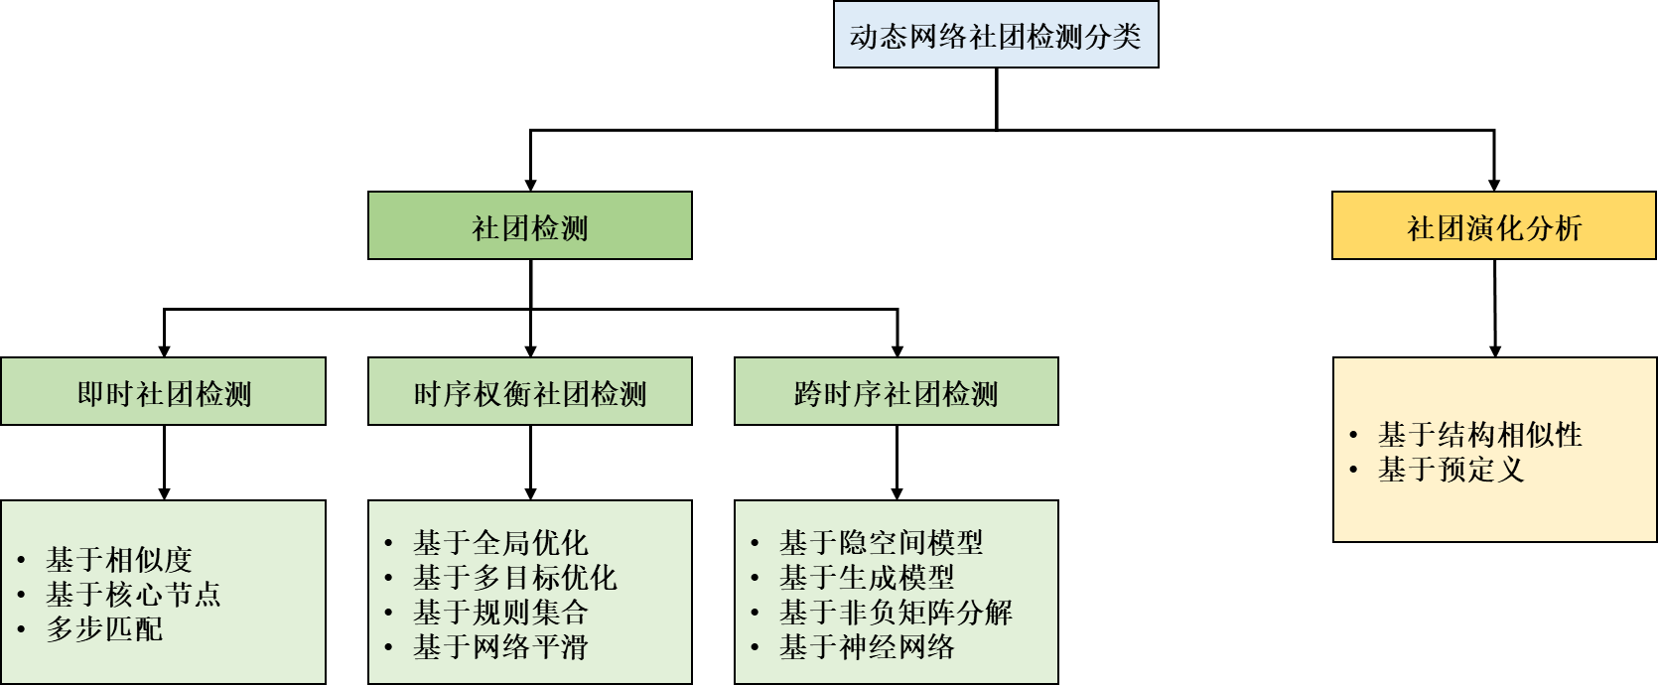
\includegraphics[width=\linewidth]{figures/chap01/classification of dcd.png}
    \caption{动态网络社团检测分类示意图}
    \label{chap1:fig:dcdclasses}
\end{figure}

\subsubsection{社团检测方法研究现状}

动态社团检测的任务核心仍然是识别每个网络快照的社团结构,根据模型对时序信息的融合思想,可以划分为即时社团检测、时序权衡社团检测与跨时序社团检测,其对时序信息的融合程度逐层递增,三类方法的优劣如表~\ref{chap1:dynamicmethod}所示。

\begin{table}[htbp]
	\caption{动态网络社团检测方法对比简表}
	\vspace{0.5em}\centering\wuhao
	\label{chap1:dynamicmethod}
	\resizebox{0.98\textwidth}{!}{
		\begin{tabular}{lp{4cm}p{3cm}p{3cm}cp{2cm}}
			\toprule[1.5pt]
			方法类别 & 核心思想 & 方法优势 & 方法不足 & 代表性工作\\
			\midrule[1.0pt]
			\textbf{即时社团检测} & 每个快照社团检测仅依赖于当前快照的网络结构,通过相似性进行跨时序社团匹配  & 可直接复用静态社团检测方法,易于并行计算,效率高 & 结果不稳定  & ~\cite{rosvall2010mapping,bota2011dynamic,falkowski2007data} \\
			\textbf{时序权衡社团检测} & 每个快照的社团结构依赖于前序快照的信息与当前快照网络拓扑 & 社团结果稳定,能够刻画社团及网络演化 & 难以并行,存在长时社团错误累积风险 & ~\cite{shang2014real,cazabet2011simulate,liu2020detecting} \\
			\textbf{跨时序社团检测} & 同时考虑所有快照的社团检测,引入超图同时建模网络拓扑与时序演化 & 社团结果稳定,受噪声影响小 & 模型复杂度较高  & ~\cite{ma2019detecting,yang2011detecting,wilson2019modeling,de2021deep} \\
			\bottomrule[1.5pt]
		\end{tabular}
	}
\end{table}

\textbf{即时社团检测方法}的主要思想旨在基于已有成熟的静态网络社团检测方法与社团匹配方法实现对动态网络的社团检测,因此该方法并未考虑动态网络演化建模问题,此类方法属于典型的“两步法”,即首先对每个快照的网络运行静态社团检测方法以得到每个快照的社团结果,随后将相邻快照的社团进行对齐,以得到动态网络社团检测结果。此类方法按照匹配思想的区别可以划分成三类,分别是基于相似度的方法、基于核心节点的方法和基于多步匹配的方法,
% 各方法对比见表~\ref{chap1:tab:instantOptimal}。

% \begin{table}[htbp]
% 	\caption{即时社团检测方法分类对比简表}
% 	\vspace{0.5em}\centering\wuhao
% 	\label{chap1:tab:instantOptimal}
% 	\resizebox{0.98\textwidth}{!}{
% 		\begin{tabular}{lp{4cm}p{3cm}p{3cm}cp{2cm}}
% 			\toprule[1.5pt]
% 			方法类别 & 核心思想 & 方法优势 & 方法不足 & 代表性工作\\
% 			\midrule[1.0pt]
% 			\textbf{基于相似度的方法} & 各快照执行静态社团检测,通过相似度度量匹配相邻快照的社团 & 方法简单,运行效率高 & 无法识别社团演化行为  & ~\cite{palla2007quantifying,rosvall2010mapping,bota2011dynamic} \\
% 			\textbf{基于核心节点的方法} & 各快照执行静态社团检测,通过中心性高的节点的社团变化进行相邻快照社团匹配 & 方法简单,能够识别社团分裂、合并行为 & 识别效果相对不稳定 & ~\cite{wang2008commtracker,chen2010detecting} \\
% 			\textbf{基于多步匹配的方法} & 各快照执行静态社团检测,匹配社团时尽可能考虑多个连续快照的社团结果 & 社团检测效果较好,可以识别社团重现 & 无法处理在线数据  & ~\cite{falkowski2006mining,falkowski2007data} \\
% 			\bottomrule[1.5pt]
% 		\end{tabular}
% 	}
% \end{table}

基于相似度匹配的方法通过定义质量函数(如Jaccard相似度)来衡量不同快照的社团的相似程度,即相邻快照的两个社团如果相似度较高(或定义阈值),则认为这两个社团在连续快照中是同一个社团。Hopcroft等人\cite{hopcroft2004tracking}首先给出了基于相似度匹配的动态社团检测方法范式,首先通过同一个静态社团检测方法检测每个快照的社团结构,随后给出相邻快照中的社团匹配函数:
\begin{equation}
    match(C,C^{'})=\min(\frac{\lvert C \cap C{'} \rvert}{\lvert C \rvert},\frac{\lvert C \cap C^{'} \rvert}{\lvert C^{'} \rvert}),
\end{equation}
其中$C$和$C^{'}$表示被匹配的两个社团内的节点集合。Pella等人\cite{palla2007quantifying}提出了以团渗透算法(CPM)进行连续快照$t$到$t+1$的社团匹配,在该文章中,作者还探讨了如何利用社团内节点的变化来预估社团存续时长,他们观察到小型社团存续的关键在于对同质性节点的吸收能力,而大型社团存续的关键则在于持续的变化。Rosvall等人\cite{rosvall2010mapping}则考虑此类方法在大规模网络的应用问题,提出了在每个快照中寻找稳定社团的方法,即通过对原始网络的每个快照进行扰动以生成多个(具体来说,进行$1000$次扰动)新的网络,并重复进行社团检测,按照人工设置的阈值将这些社团结果进行合并进而形成稳定社团。在后续的工作中,Asur等人\cite{asur2009event}则提出了可以在社团匹配步骤中通过改进社团匹配函数来实现对动态网络社团演化行为的识别,并获得了一定发展\cite{bota2011dynamic}。

基于核心节点的方法则认为网络中具有较高权重的节点能够左右社团在时序的变化,因此在社团匹配过程中,如果相邻快照中的两个社团存在同一个中心性指标较高的节点,则这两个社团在连续快照中是同一个社团。这种方法相较于相似度匹配的方法能够识别社团的分裂或者合并行为,因为一个社团中可能存在多个核心节点,这些节点的社团转移并不一定相同。Wang等人\cite{wang2008commtracker}首先提出了此类方法的范式,并提出了一个投票策略来识别各个快照的社团中的核心节点。Chen等人\cite{chen2010detecting}在此基础上进行了优化,他们采用了社团的保守定义,即图中的最大团,来缩小社团匹配步骤的搜索域,提升效率的同时避免了冗余社团,并定义了代表社团的核心节点应该在同一快照中出现在其他社团频次最少。

多步匹配方法则并不仅考虑相邻快照的社团匹配,而是同时考虑多个相邻快照(尽可能远的)的社团匹配问题,匹配方法可以是基于相似度匹配或者基于核心节点的方法。此类方法能够识别社团重现,但难以实现在线运行,因为多步匹配可能在新快照加入后使得前序快照的社团结果发生改变。Falkowski等人\cite{falkowski2006mining,falkowski2007data}定义了多步匹配的核心思想,即根据社团相似性度量$overlap(x,y)=\frac{\lvert x \cap y \rvert}{min(\lvert x \rvert,\lvert y \rvert)}$将多个相邻快照中的相同社团进行关联,以得到社团存续图,随后在社团存续图中再次执行静态社团检测算法来获得多个快照的社团关联性。

即时社团检测的基本思想使得此类方法在识别社团结构时并不考虑时间信息对社团检测结果的影响,这使得此类方法受噪声影响较大,且社团检测结果不稳定,虽然以Rosvall等人\cite{rosvall2010mapping}为代表的部分学者利用策略获得稳定社团或通过缩紧社团定义以解决这些问题,但并未从本质上改变此类方法的短板。另外,此类方法在忽略社团检测效果的前提下,对于社团生命周期的检测也取得了一定的成果\cite{chen2010detecting},这也为社团演化分析任务提供了方法支撑。
 
\textbf{时序权衡社团检测方法}考虑到了在动态社团检测任务中,前序快照对当前快照的影响,在进行当前快照社团检测时,需要权衡前序快照社团结构与网络演化对当前快照社团检测的影响,但并不考虑未来快照对当前快照的影响,这也是此类方法能够实现在线社团检测的前提,称为进化聚类。此类方法可以总结为两个迭代步骤,首先对动态网络第一个快照的网络执行社团检测,随后对后续快照按时序在结合前序快照社团结构的前提下逐个识别社团结构。按照方法的不同,此类方法可以进一步划分成基于全局优化、基于多目标优化、基于规则集合和基于网络平滑的方法。基于全局优化和基于多目标优化的方法主要基于前序快照的社团结构与当前快照与前一快照的网络图谱变化来更新社团结果;而基于规则集合和基于网络平滑的方法则在对当前快照进行社团检测时考虑前序快照的信息。
% 各方法对比见表~\ref{chap1:tab:instantOptimal}。

% \begin{table}[htbp]
% 	\caption{即时社团检测方法分类对比简表}
% 	\vspace{0.5em}\centering\wuhao
% 	\label{chap1:tab:instantOptimal}
% 	\resizebox{0.98\textwidth}{!}{
% 		\begin{tabular}{lp{4cm}p{3cm}p{3cm}cp{2cm}}
% 			\toprule[1.5pt]
% 			方法类别 & 核心思想 & 方法优势 & 方法不足 & 代表性工作\\
% 			\midrule[1.0pt]
% 			\textbf{基于全局优化的方法} & 各快照执行静态社团检测,通过相似度度量匹配相邻快照的社团 & 方法简单,运行效率高 & 无法识别社团演化行为  & ~\cite{palla2007quantifying,rosvall2010mapping,bota2011dynamic} \\
% 			\textbf{基于规则集合的方法} & 各快照执行静态社团检测,通过中心性高的节点的社团变化进行相邻快照社团匹配 & 方法简单,能够识别社团分裂、合并行为 & 识别效果相对不稳定 & ~\cite{wang2008commtracker,chen2010detecting} \\
% 			\textbf{基于多目标优化的方法} & 各快照执行静态社团检测,匹配社团时尽可能考虑多个连续快照的社团结果 & 社团检测效果较好,可以识别社团重现 & 无法处理在线数据  & ~\cite{falkowski2006mining,falkowski2007data} \\
% 			\bottomrule[1.5pt]
% 		\end{tabular}
% 	}
% \end{table}
基于全局优化的方法主要以社团聚类质量函数为衡量指标(如模块度、传导率等),以$t$时刻的社团检测结果为起点,迭代地将$t+1$时刻的节点更换社团归属以最大化质量函数,从而达到识别$t+1$时刻社团的目的。Miller等人\cite{miller2010continuous}参考潜在狄利克雷分配过程(Latent Dirichlet Allocation,LDA)设计了动态图主题模型,将社团视作随时序演化的主题,节点之间的连边则对应文档中的词汇,通过前一个快照的主题来初始化当前快照的主题,通过这种方法实现了对动态网络时序演化的建模与社团检测。Aynaud等人则利用模块度优化方法来实现对动态网络社团演化的建模,首先在第一个快照上运行Louvain算法识别其社团结构,随后通过在后续快照中改变节点的社团划分来优化模块度,使模块度达到局部最优,为了保证社团稳定性,$t$时刻的社团结构初始化由$t-1$时刻确定。G{\"o}rke等人\cite{gorke2010modularity}在社团初始化设置的基础上添加了回溯策略以提升$t$时刻社团的搜索空间。Shang等人\cite{shang2014real}则进一步提出了在动态社团检测过程中,在对$t$时刻快照进行社团检测之前,引入网络修剪策略来尽可能将$t$时刻的网络结构的拓扑噪声进行剔除。  

基于规则集合的方法考虑在前序快照和当前快照之间发生的网络变化(边/节点的出现或消失),定义一系列规则来确定网络变化如何更新当前快照的社团。Falkowski等人\cite{falkowski2008studying}基于经典的DBSCAN方法提出了DENGRAPH算法,该方法定义了一个新的临近性指标,其定义了节点对之间的距离。当节点$u$和$v$的临近性超过阈值时,称节点$u$和$v$密度可达。当节点$u$具有超过$\eta$个密度可达邻居时,则称$u$为核心节点。社团由密度可达的核心节点的集合组成。通过定义上述规则,该算法可以根据动态网络快照的节点和边的变化快速更新动态网络社团结构,其社团定义较一般社团的定义更为严格。Nguyen等人\cite{nguyen2011adaptive}则提出了QCA算法,设计一系列的规则函数来根据动态网络前一个快照的网络结构变化(节点/边的添加和消失)更新当前快照的社团划分。Cazabet和Amblard\cite{cazabet2011simulate}则从强化学习的角度提出了基于多agent的社团检测方法,其将动态网络视作环境变量、社团视作环境中的agent,当环境发生改变,则通过策略集中定义的规则对社团结果进行更新。

基于多目标优化的方法则同时考虑了当前社团检测效果与当前快照和前序快照之间的时序平滑性,因此其定义了优化范式来融合两个优化目标:
\begin{equation}
c=\alpha CS+(1-\alpha CT),
\end{equation}
其中$CS$表示当前快照的社团检测效果,$CT$表示时序平滑性效果,$\alpha$则表示二者的权重。Zhou等人\cite{zhou2007discovering}首先提出基于正则化割是被每个快照的社团,并引入额外的距离函数衡量当前快照社团划分与前序快照社团划分之间的差距,通过多目标优化范式平衡当前社团结果与前序社团结果的最优化以获得动态网络社团结果。Folino等人\cite{folino2013evolutionary}在多目标优化框架下引入了遗传算法,第一个目标函数用来提升当前快照的社团检测结果,第二个目标通过最大化当前快照与前一快照的正则化标准互信息(NMI)来确保网络平滑性。Sun等人\cite{sun2013co}通过狄利克雷过程混合模型实现对动态网络的社团生成,利用吉布斯采样对模型参数进行推断求解,其社团发现由当前快照的最优社团与前序快照的演化平滑之间进行平衡。Liu等人\cite{liu2020detecting}考虑动态网络社团演化行为的变化引入了社团迁移操作符来细化动态网络社团演化模式。

基于网络平滑的方法则通过考虑过去网络的变化来优化当前快照的网络拓扑,例如按照前序网络变化来对当前快照的网络结构增加或删除边,以此将网络平滑性融入到当前快照中,进一步在平滑后的当前快照中执行社团检测算法。Guo等人\cite{guo2014evolutionary}基于模块度优化方法设计了基于网络平滑的动态网络社团检测算法,其对当前快照的网络结构与前一快照的网络结构进行融合,形成trade-off邻接矩阵,并在该邻接矩阵中进行静态社团检测以获得动态社团划分结果。Xu等人\cite{xu2013community}则设计了更加精细的更新策略,通过设计\textit{累积稳定边}来得到动态网络演化过程中相对稳定的结构,并在此结构上进行社团检测,以此获得稳定的动态社团划分。

时序权衡社团检测方法通过不同的设计思路来平衡各快照的最优社团结果与时序平滑性对动态社团检测的影响。此类方法由于考虑了时序平滑性,因此能够产生在时序过程中稳定的社团结果。但由于对动态网络每个快照进行社团检测时需要考虑前序快照或多个前序快照的信息,因此此类方法难以并行计算。另外,由于对动态网络时序平滑的引入,此类方法可能存在社团结果的错误累积,导致长时间序列的动态网络社团检测结果逐渐失真。


\textbf{跨时序社团检测方法}则将动态网络的演化与动态社团检测进行融合,以获得更加全局的动态网络社团检测结果。此类方法的社团检测效果主要取决于对于动态网络演化建模的有效程度,也是当前动态社团检测的主流思想。此类方法按照方法不同可以划分为基于非负矩阵分解的方法、基于隐空间模型的方法、基于生成模型的方法和基于神经网络的方法。

非负矩阵分解方法进行社团检测的核心思想是利用非负矩阵对网络拓扑的低维分解等价于聚类方法的原理,通过设计模型将动态网络演化模式融入到模型中以达到对动态网络演化建模及社团检测的目的\cite{KXTS202104002}。Lin等人\cite{lin2009analyzing}提出的FacetNet算法,在$t$时刻的社团检测通过引入混合模型来实现,而对于动态网络平滑则通过计算当前快照与前序快照的KL散度实现,提升了模型的鲁棒性。而FacetNet通过非负矩阵分解的技术路线将网络演化与社团检测进行了联合建模,使得该模型能够将网络演化建模与社团检测进行融合。Gao等人\cite{gao2017dynamic}提出的ENMF则参考动态随机块模型(DSBM)\cite{yang2011detecting}引入了社团转移矩阵来显式地刻画动态网络的演化,可以在保证社团检测效果的前提下支持动态网络演化分析。Ma等人\cite{ma2017evolutionary}则证明了ENMF与动态谱聚类方法在理论上是等价的,并基于该证明将谱聚类引入到ENMF框架中,提升了该模型的社团检测效果。Ma等人\cite{ma2019detecting}在后续工作中进一步引入了图正则项将动态网络历史快照的结构融入到当前快照社团检测任务中,在保证复杂度不增的前提下进一步提升了社团检测效果。

隐空间模型则认为复杂网络的演化受到高维空间的影响,因此可以通过将动态网络的节点或边组成的拓扑结构映射到高维空间中,并在高维空间建模动态网络的演化。在此过程中将社团结构融入到模型中来同步获得动态网络社团划分。Sewell等人\cite{sewell2015latent}首先提出了动态隐空间模型的范式,即通过将节点映射到高维隐空间中来表示节点在网络中的位置(类似于网络表示学习),并利用节点高维空间相似性聚类实现社团检测,并利用隐马尔可夫模型建模社团在高维隐空间中的演化模式,随后利用MCMC采样实现对社团求解。Liu等人\cite{liu2022variational}则引入了变分推断的方法来对隐空间模型参数进行求解,提升了模型的运行效率。Daniel等人\cite{daniel2023bayesian}则针对动态隐空间模型在高维空间中的时序演化机制进行了细化,通过引入层次狄利克雷隐马尔可夫模型显式地建模了社团的分裂合并等行为。

生成模型则在隐空间模型的概念上更进一步,通过设计动态网络的生成机制,并将社团结构纳入到生成机制中(即认为动态网络的节点和边的生成及演化受到社团的影响),通过对该生成机制的模型参数求解以获得动态网络社团划分。其中最经典的方法是Yang等人\cite{yang2011detecting}提出的动态随机块模型(DSBM),该模型通过引入社团转移矩阵来显式地建模了动态网络社团的演化,并沿用了经典随机块模型的网络生成机制,即节点的连边仅与节点所在社团有关。在此基础上进一步提出假设,节点的社团划分的演化仅与其所在社团与社团转移矩阵有关。DSBM提出了模型参数的两种推断方法,分别是基于共轭先验的参数后验推断与EM算法,并给出了在线和离线两个版本的模型。Tang等人\cite{tang2014detecting}在此基础上考虑DSBM无法实现动态社团模型选择的问题,提出了基于狄利克雷过程的动态随机块模型,通过狄利克雷过程自动确定动态网络社团个数。Xu\cite{xu2015stochastic}则对DSBM的演化所依赖的隐马尔可夫假设进行了改进,允许前序边的变化直接影响当前快照边的生成,并提出了结合卡尔曼滤波和局部搜索的求解策略。Wilson等人\cite{wilson2019modeling}引入了度异质性参数来对DSBM进行了改进,实现了随机块模型对节点的度异质性进行捕获。

基于神经网络的方法则普遍将动态网络建模与社团检测任务切分开来,利用图神经网络将动态网络各快照中的拓扑与属性信息进行解耦,形成节点的低维表示,并在节点表示向量中利用聚类算法获得社团结构,代表性的方法包括基于GCN的方法\cite{ma2020streaming,pareja2020evolvegcn}、基于GAT的方法\cite{cui2019hierarchical}、基于AE的方法\cite{goyal2018dyngem,yu2018netwalk,zhao2019large,goyal2020dyngraph2vec}等。上述方法的创新点均是为了模型能够更好地捕获动态网络的属性或拓扑信息以获得节点的表示向量,而执行社团检测任务往往通过对节点表示向量执行聚类操作实现,这种“两步法”的方式虽然效率较高,但所获得的聚类结果本质上是相似节点的集合,并不能直接代表动态网络的社团结构。Santo等人\cite{de2021deep}则通过基于CNN的稀疏卷积设计,同时引入部分社团真相实现了对动态网络社团的半监督学习,但社团本质是无监督任务,引入社团真相一定意义上无法在实际应用中起到作用。Yao等人\cite{yao2021interpretable}则通过改进动态网络快照的网络结构,引入衰减参数将前序快照与当前快照网络结构进行融合,通过神经网络学习网络表示,并引入谱聚类获得社团结构,该方法还证明了此种改进理论上与DSBM近似。由于神经网络属于经典的黑盒模型,即使其针对动态社团检测任务进行了优化,模型参数也无法理解,难以应用到社团演化分析任务中。

跨时序社团检测方法的核心是更好地实现动态网络演化模式的建模,因此此类方法往往能够适应更多的动态网络下游任务,如链接预测、异常检测、演化分析等。并且此类方法中,生成模型、隐空间模型及非负矩阵分解方法的模型隐变量均具备一定的物理或现实意义,故其具有良好的可解释性,其中以生成模型的可解释性最好,能够支撑更深入的网络演化分析及挖掘任务,但往往复杂的模型架构与模型推断复杂导致上述模型难以适用于大规模网络。而基于神经网络的方法往往由于其黑盒特性而缺乏可解释性,因此难以用于社团演化分析研究。




\subsubsection{社团演化分析研究现状}

社团演化分析任务的核心是通过挖掘动态网络社团随时间的变化模式,以揭示社团结构的时序演化规律,支持人们对复杂系统的因果关系理解与推断、预测以及控制。对社团演化的分析可以帮助提升复杂系统的鲁棒性与韧性。动态网络社团演化分析的相关方法按照设计思路可以划分为基于结构相似性的方法和基于预定义的方法。方法对比见表~\ref{chap1:tab:ievolution}

\begin{table}[htbp]
	\caption{社团演化分析方法分类对比简表}
	\vspace{0.5em}\centering\wuhao
	\label{chap1:tab:ievolution}
	\resizebox{0.98\textwidth}{!}{
		\begin{tabular}{lp{4cm}p{3cm}p{3cm}cp{2cm}}
			\toprule[1.5pt]
			方法类别 & 核心思想 & 方法优势 & 方法不足 & 代表性工作\\
			\midrule[1.0pt]
			\textbf{基于结构相似性的方法} &通过定义相邻快照的相似性指标来识别社团的时序演化关系 & 指标相对直观,易于理解 & 泛化能力差,可解释性较差  & ~\cite{palla2007quantifying,zhong2014evolution,wang2024community} \\
			\textbf{基于预定义的方法} & 通过预定义动态网络中的演化事件,并定义阈值来进行动态网络事件检测 & 扩展性强,理解直观,可帮助预测社团未来行为 & 依赖人工定义的指标,缺乏统一标准 & ~\cite{greene2010tracking,brodka2013ged,mazza2023modularity,zhao2023dynamic} \\
			\bottomrule[1.5pt]
		\end{tabular}
	}
\end{table}

\textbf{基于结构相似性的方法}的基本假设认为动态网络每个快照的社团结构已经获得,通过定义相邻快照的相似性指标并定义阈值来识别社团在时序上的演化关系,进而分析社团的演化模式。Palla等人\cite{palla2007quantifying}通过团渗透的方法获得了动态网络的社团结构,进而定义了社团在不同快照中的自相关函数以及社团稳定性指标,通过对论文合作网络与通信网络的分析,得到不同规模社团的演化规律,即大规模社团变动频繁、小规模社团相对稳定。Zhang等人\cite{zhong2014evolution}针对物联网网络的演化,提出了基于模块度增益的社团演化分析方法,并引入了正则化互信息指标与自相关函数来衡量社团稳定性。Wang等人\cite{wang2024community}考虑物理系统的鲁棒性,通过定义广义介数中心性模型与网络负荷流模型来模拟通信网络和电力网络在演化过程中的鲁棒性,该模型考虑了社团结构在网络演化中的作用,并总结出社团边缘的节点变动对网络鲁棒性影响较大。
基于结构相似性的方法以定义网络演化相似性度量实现对动态网络与动态社团演化的建模与分析,这种方式依赖于指标设计与社团检测效果,且其模型往往缺乏可解释性,不具备指标外的泛化能力。


\textbf{基于预定义的方法}则将社团演化行为视为网络中的各种事件,通过识别网络中的预定义事件的模式来分析动态网络及动态社团的演化。Greene等人\cite{greene2010tracking}提出了一种可扩展的社团演化事件识别方法,通过定义社团诞生、死亡、合并、分裂、扩展、收缩事件,并设计一系列阈值进行匹配来实现对社团演化事件的识别。Br{\'o}dka等人\cite{brodka2013ged}则进一步将社团演化事件扩展成$8$种,并定义了社团归属指标$I$来衡量两个社团的相似性,基于该指标进一步定义了一系列的阈值进行社团演化事件的识别。Mazza等人\cite{mazza2023modularity}则提出了无阈值框架,通过将所识别的社团结构视为节点,社团间的相似性视为边构建了社团相似性网络,并在该网络中进行模块度优化聚类,用聚类结果实现动态网络社团演化分析。Zhao等人\cite{zhao2023dynamic}则在考虑人类移动的空间平滑性更新了上述社团演化事件的定义,并将其应用在城市人类移动分析中。
基于预定义的方法往往以预定义的事件及事件特征为基准,通过设定阈值识别网络中的事件,其对动态网络及动态社团的演化分析比较直观,但且缺乏统一标准,需要人工信息指导。

总的来说,动态网络社团演化分析方法往往依赖于社团检测准确性,难以完全脱离动态社团检测任务而独立存在。

\section{研究内容与创新点}

本文以动态复杂网络为研究对象,从动态网络社团检测与演化分析任务出发,重点关注动态网络的生成机制建模与分析,从随机块模型的角度构建动态网络的高阶生成机理,从实证分析出发,解决生成模型在动态网络演化机制中的社团与节点的演化异质性缺失问题,以提升随机块模型对动态网络演化模式的建模能力与演化分析能力,并结合图神经网络与深度序列模型探索了动态社团检测的深度生成建模方法,为动态社团检测的大规模数据可解释性建模提供基础。
从研究目标上,以随机块模型为理论基础,针对真实世界动态网络数据挖掘动态网络的高阶生成机理,以支撑动态网络演化模式改进;针对动态随机块模型对节点演化异质性生成建模缺失的问题进行改进,提出动态网络的微观节点-介观社团-宏观网络快照的层次狄利克雷生成框架,扩展动态随机块模型的建模深度;从动态随机块模型的动态网络演化分析出发,提出动态网络层次演化异常识别指标,扩展动态随机块模型的动态网络演化分析深度;针对动态随机块模型参数量过高,难以针对大规模数据进行应用的问题,提出动态网络深度生成模型社团检测建模,解决深度学习模型的黑盒问题同时,为动态网络生成模型的大规模应用提供方法范式。其研究思路及主要研究内容关系如图~\ref{chap1:fig:framework}所示:
\begin{figure}
    \centering
    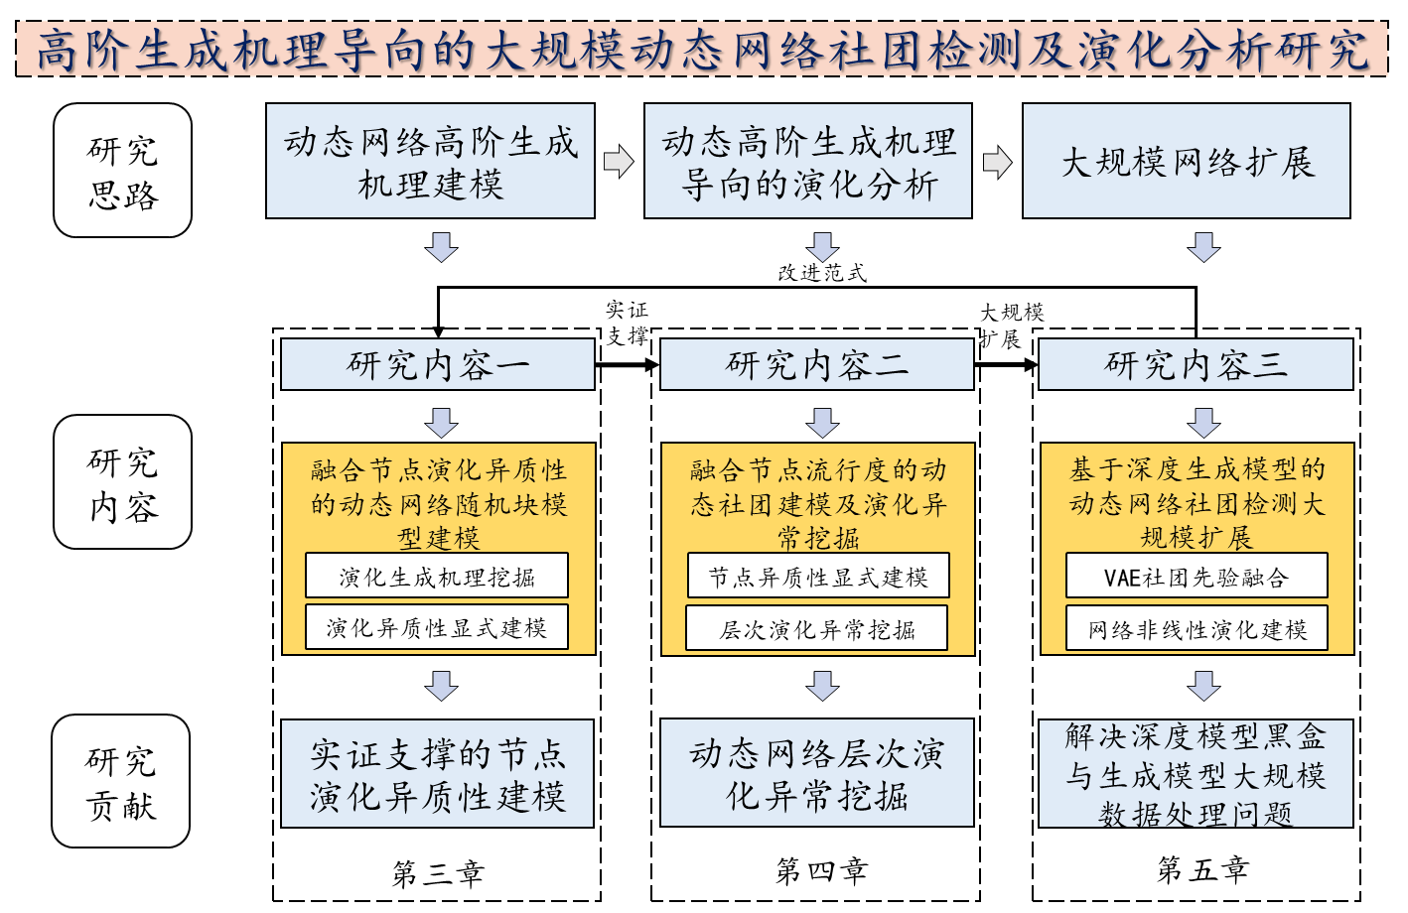
\includegraphics[width=.75\linewidth]{figures/chap01/framework.png}
    \caption{本文研究思路及关联}
    \label{chap1:fig:framework}
\end{figure}

第一,提出动态网络高阶生成机理挖掘框架,探索动态网络节点变化与社团演化之间的本质关联。考虑到动态网络的演化由节点和边的变化驱动,而社团的演化则由节点的社团归属变化而驱动,因此需要明确动态网络中节点演化与社团演化的相互作用关系。在其指导下,研究融合动态网络高阶生成模式的动态随机块模型。针对经典随机块模型对动态网络生成机理建模能力提升的问题,设计生成机制,进一步地提升动态随机块模型的建模能力,并研究有效的动态随机块模型参数推断方法,进而研究该模型在社团检测与社团演化分析的有效性。

第二,研究动态随机块模型社团演化分析的深入挖掘方法。在研究内容一的基础上,改进并简化动态随机块模型的建模方法,提升模型参数的可解释性与易理解性,研究基于动态随机块模型的动态网络各层次演化异常定义以提升动态随机块模型的社团演化分析能力,并在真实数据中验证其有效性。

第三,针对动态随机块模型难以大规模应用问题,研究基于深度学习的动态社团深度生成建模方法。以生成模型为出发点,基于深度生成模型的框架研究生成模型参数的变分自编码器求解方法,并验证模型的动态社团检测能力及其参数的动态社团演化分析能力与大规模数据应用能力。

针对以上研究内容,本文从动态网络演化建模的角度,深入分析并提出了解决方法,取得了一定研究成果,并通过实证分析验证了提出方法的贡献。其主要贡献和创新点包括一下几个方面:

第一,本文采用特征工程的方法,将动态网络节点的社团转移行为定义成相邻快照节点是否转移的二分类问题,并提取动态网络各快照中节点与社团的属性信息,基于决策树分类实现对节点在动态网络演化过程中的高阶生成机制挖掘,通过收集大量真实世界动态网络数据进行横向对比,应用不同的经典社团检测方法剔除社团检测方法的纵向影响,最终得出结论,即动态网络的生成过程中,节点的异质性起到最主要作用。这为后续模型设计提供了实证依据。

第二,在研究内容一的支撑下,本文提出建模动态网络节点-社团演化机制的层次狄利克雷生成结构,基于动态随机块模型的基本假设,进一步引入节点级别的社团转移参数,并定义了社团转移参数与节点级别的社团转移参数的生成关系。通过变分推断方法对所提出模型进行参数后验推断,以估计模型参数拟合结果。通过在生成数据集与真实数据集的社团检测、社团演化与节点演化实验,验证了所提出方法对网络高阶生成机理建模的有效性和可行性,并挖掘了论文引用网络中节点与社团演化的规律。

第三,考虑到动态随机块模型对网络生成机制的显式建模能力,本文提出了融合节点流行度的动态随机块模型以同时建模节点拓扑异质性与演化异质性,根据该模型参数和隐变量的实际意义提出了面向微观节点、介观社团以及宏观网络快照的演化异常识别指标,拓展模型的动态网络演化分析能力,通过对真实世界数据的实验验证了本模型对动态网络及动态社团的建模能力与所提出的动态网络层次演化异常指标的有效性。

第四,针对生成模型对动态网络生成及演化的可解释性建模能力强但算法效率低、模型求解方法复杂,以及动态网络深度模型建模相对简单且运行效率高(易于优化)但黑盒特性限制其对真实世界动态网络演化分析能力的问题,提出结合二者优势的深度生成模型,根据变分自编码器与生成模型变分推断求解的理论关联,提出融合变分自编码器与混合高斯的动态网络深度社团检测算法,并利用深度序列模型建模动态网络演化。针对生成数据集与真实数据集的实验验证了所提出方法的有效性以及基于深度生成模型的动态网络演化模式挖掘的可行性,为后续动态网络社团检测算法的推广与应用提供了有效的建模框架。

\section{论文组织结构}
本文对动态社团生成机制及其深度建模问题展开研究并提出了三个工作,全文的章节结构如下所示:



第一章,主要介绍了动态网络社团检测的研究背景和意义,指出了本文的研究问题,分析了当前国内外的研究现状和挑战,随后对本文研究内容进行阐述。

第二章,介绍了本文的相关研究基础,包括动态网络社团检测相关研究技术与前沿方法,包括其研究思路以及优缺点,进一步介绍了基于深度学习的动态网络社团检测方法的相关技术路线以及深度生成模型的相关基础。

第三章,针对动态网络社团演化与节点演化的关联性设计研究框架,利用大量真实世界数据进行动态网络高阶生成机理的规律挖掘,并在此实证基础上提出融合节点演化异质性的动态随机块模型,随后介绍了模型的变分推断估计方法与实验结果及实证分析。

第四章,针对动态随机块模型的演化分析能力提升,首先提出融合节点流行度的动态随机块模型以提升模型的可解释性,随后介绍基于模型参数的动态网络、社团、节点的各层次演化异常指标,最后介绍实验以验证模型与所定义指标的有效性并进行实证分析。

第五章,针对生成模型可解释性强但模型推断复杂难以应用于大规模数据的问题与基于深度模型的方法可解释性差但方法设计简单且运行效率高的问题,提出了基于深度生成模型的动态网络深度社团检测算法,随后介绍模型实验以验证所提出方法能够融合深度模型与生成模型的优势,验证了所提出方法在动态网络演化分析的应用潜力。

第六章,总结与展望,对本文的工作和贡献进行了总结,并展望未来的研究思路。



